%!TEX encoding = UTF-8 Unicode
\documentclass{reqenglecture}

\title{Introduction to Software Requirements Engineering}

\subtitle{Part II: Functionality}

\author{Björn Regnell}

\date{\vspace{1em}\footnotesize Updated: \today~
\\ License: CC-BY-SA 
\\ \url{https://github.com/bjornregnell/reqeng-book} 
}

%\beamerdefaultoverlayspecification{<+->} %de-comment if you want pause after items

\begin{document}
\maketitle

\begin{frame}
\frametitle{Part II: Functionality}
\framesubtitle{Outline}
\tableofcontents
\end{frame}


\LectureOnly{\section{Modeling}}

\begin{Slide}{Requirements Modeling}

A requirements model...

\begin{itemize}
\item  is an informative \textbf{representation} of the intended system.

\item is an \textbf{abstraction} of the intended system 
\begin{itemize}
\item only \textit{some} aspects are represented, 
\item while other aspects are \textit{excluded}.

\end{itemize}
\item captures important knowledge gained from \textbf{elicitation}.

\item is often textual or a diagram, or both.

\item is often part of a \textbf{specification}.

\item should be \textbf{validated} by (some) stakeholders.

\end{itemize}
\end{Slide}

\begin{Slide}{Different aspects of requirements to model }

\begin{minipage}[t]{0.6\textwidth}
\begin{itemize}
\item Functional aspects:
\begin{itemize}
\item Data aspects:
\begin{itemize}
\item What is stored and processed by the system?
\item What is the format of input and output data?

\end{itemize}
\item Business Logic aspects: 
\begin{itemize}
\item How should the system behave in different usage contexts?
\item What output should be produced, given input and state?  
\end{itemize}
\end{itemize}
\end{itemize}
\end{minipage}%
\begin{minipage}[t]{0.4\textwidth}
\vspace{0.0em}\hfill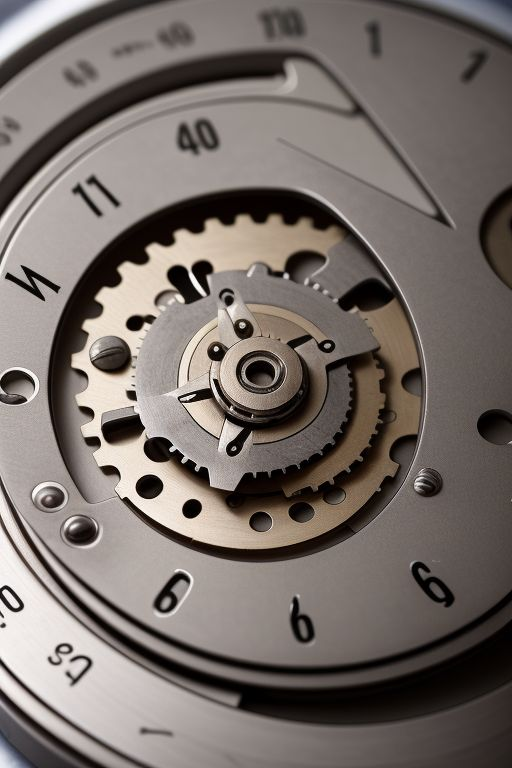
\includegraphics[width=0.82\textwidth]{../img/cog1}
\end{minipage}%

\begin{itemize}
\item Quality aspects: 
\begin{itemize}
\item What is a 'good' function from stakeholders' viewpoints?
\item More on quality modeling in Part III.

\end{itemize}
\end{itemize}
\end{Slide}

\begin{Slide}{Which modeling technique is best? }

\begin{itemize}
\item A modeling technique may be more or less suitable for representing some aspects of requirements from some stakeholders' viewpoint.

\item A \textbf{well-balanced combination} of modeling techniques can capture a more aspects in a better way than a single technique.

\item What modeling technique is best depends on...
\begin{itemize}
\item abstraction level
\item project type
\item stakeholders
\item tool support
\item the number and kind of requirements
\item ...

\end{itemize}
\item Model interpretation often requires specific knowledge: 
\begin{itemize}
\item Choose modeling technique based on stakeholders' ability to understand and validate!

\end{itemize}
\item How do you know that your chosen mix of models fit together and does not contradict each other?
\begin{itemize}
\item Make sure to check model inter-consistency in validation!

\end{itemize}
\end{itemize}
\end{Slide}
\LectureOnly{\section{Data}}
\begin{Slide}{Data Modeling }
\begin{itemize}
\item Functional modelling techniques with focus on \textbf{data}:
\begin{itemize}
\item \textbf{Data dictionaries}: 
\begin{itemize}
\item a list of data types with textual description of each field and relations to other data types
\end{itemize}
\item \textbf{Data windows}: 
\begin{itemize}
\item examples of instances of data types shown in a usage context
\item often shown as a screen mockup
\item often \textit{not} intended for interface design; instead the focus is on specification and validation of stored and processed data 
\end{itemize}
\item \textbf{Data diagrams}: 
\begin{itemize}
\item boxes and arrows with data types, their fields and relations  
\item Entity-Relationship-diagrams
\item Class diagrams

\end{itemize}
\end{itemize}
\end{itemize}
\end{Slide}
\LectureOnly{\section{Business Logic}}

\begin{Slide}{Business Logic Modeling}
\begin{itemize}
\item TODO

\end{itemize}
\end{Slide}
\begin{Slide}{next slide}
\begin{itemize}
\item TODO
\begin{itemize}
\item blabla
\end{itemize}
\end{itemize}
\end{Slide}
\end{document}